\chapter{Remote photoplethysmography: non-contact heart rate measurement}
\label{ch:literature-rppg}

Photoplethysmography (PPG) is a technique commonly used to measure HR based on the variations of light absortion in the human skin. The pressure of the cardiac activity causes the blood vessels to change volume and light absorbtion rate because of the levels of oxigen in the blood flow. Such differences make the light absorption on the skin surface change accordingly. PPG is a time-varying signal resulted from such differences in the light absorption in live human tissue, which can be processed to calculate the HR. The process is illustrated in Figure \ref{fig:ppg}. The employment of PPG requires a physical sensor, e.g. finger pulse oximeter, in order to be performed.

\begin{figure}[h]
\centering
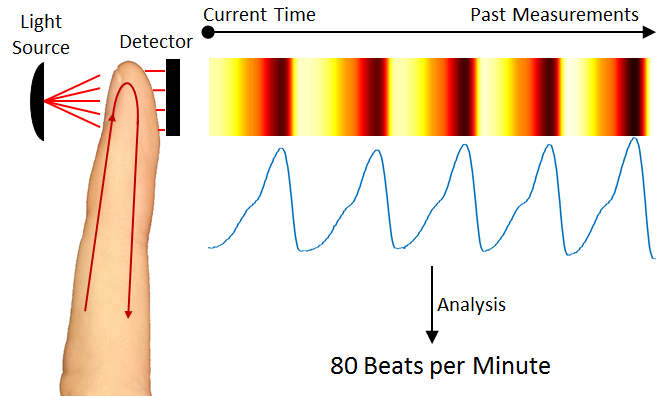
\includegraphics[width=0.6\linewidth]{Content/figures/ppg.png}
\caption{General structure of a physical photoplethysmographic system. Adapted from \textcite{chwyl2016statistical}.}
\label{fig:ppg}
\end{figure}

Further research on PPG \parencite{mcduff2015survey} evolved the technique to allow it to be performed remotely based on the analysis of a video of a person. The remote approach is commonly refered in the literature as remote photoplethysmography (rPPG)  \parencite{allen2007photoplethysmography}. Such improvement removed the requirement of a physical sensor or any physical contact for the estimation of HR and its derivates. A literature review shows the existence of a variety of different rPPG approaches, including thermal-, image-, and movement-based ones \parencite{kranjec2014non, Sereevoravitgul}. The following sections present the common structure of an rPPG technique, a survey of existing rPPG techniques and information regarding accuracy and limitations of such technology.

%rPPG-based methods for HR measurement are tools that can be used by the HCI community, particularly in games research.

%The use of physiological signals to infer information about users is a recurrent research topic \parencite{kivikangas2011review,jerritta2011physiological, kukolja2014comparative}. However the methods employed to obtain such signals are commonly based on physical contact, e.g. ECG, and few initiatives have been carried out relying on non-contact approaches, e.g. rPPG. In the computer vision domain, on the other hand, an increasing number of works is concerned with creating new (or improving already existing) techniques for rPPG. To provide an introduction for readers unfamiliar with rPPG, we introduce its general structure and the core techniques in the field. Additionally we present works involving physiological signals, in particular HR, and game-related materials commonly used for detection of emotional states of users.

%%%%%%%%%%%%%%%%%%%%%%%%%%%%%%%%%%%%%%%%%%%%%%%%%%%%%%%%%%%%%%%%%%%%%%%%%%%%%%%%%%%%%%%%%%%%%%%%%%%%%%%
\section{Structure of the technique}
\label{sec:literature-rppg-structure}
%%%%%%%%%%%%%%%%%%%%%%%%%%%%%%%%%%%%%%%%%%%%%%%%%%%%%%%%%%%%%%%%%%%%%%%%%%%%%%%%%%%%%%%%%%%%%%%%%%%%%%%

There exist initiatives to classify \parencite{rouast2016remote, mcduff2015survey} and formally model the algorithmic principles \parencite{Wang_2016algorithmic} of rPPG techniques. In that light, \textcite{rouast2016remote} propose a general algorithm framework composed of three phases that are common to all rPPG techniques (see Figure \ref{fig:rppg}): signal extraction, signal estimation and heart rate estimation.

\begin{figure}
\centering
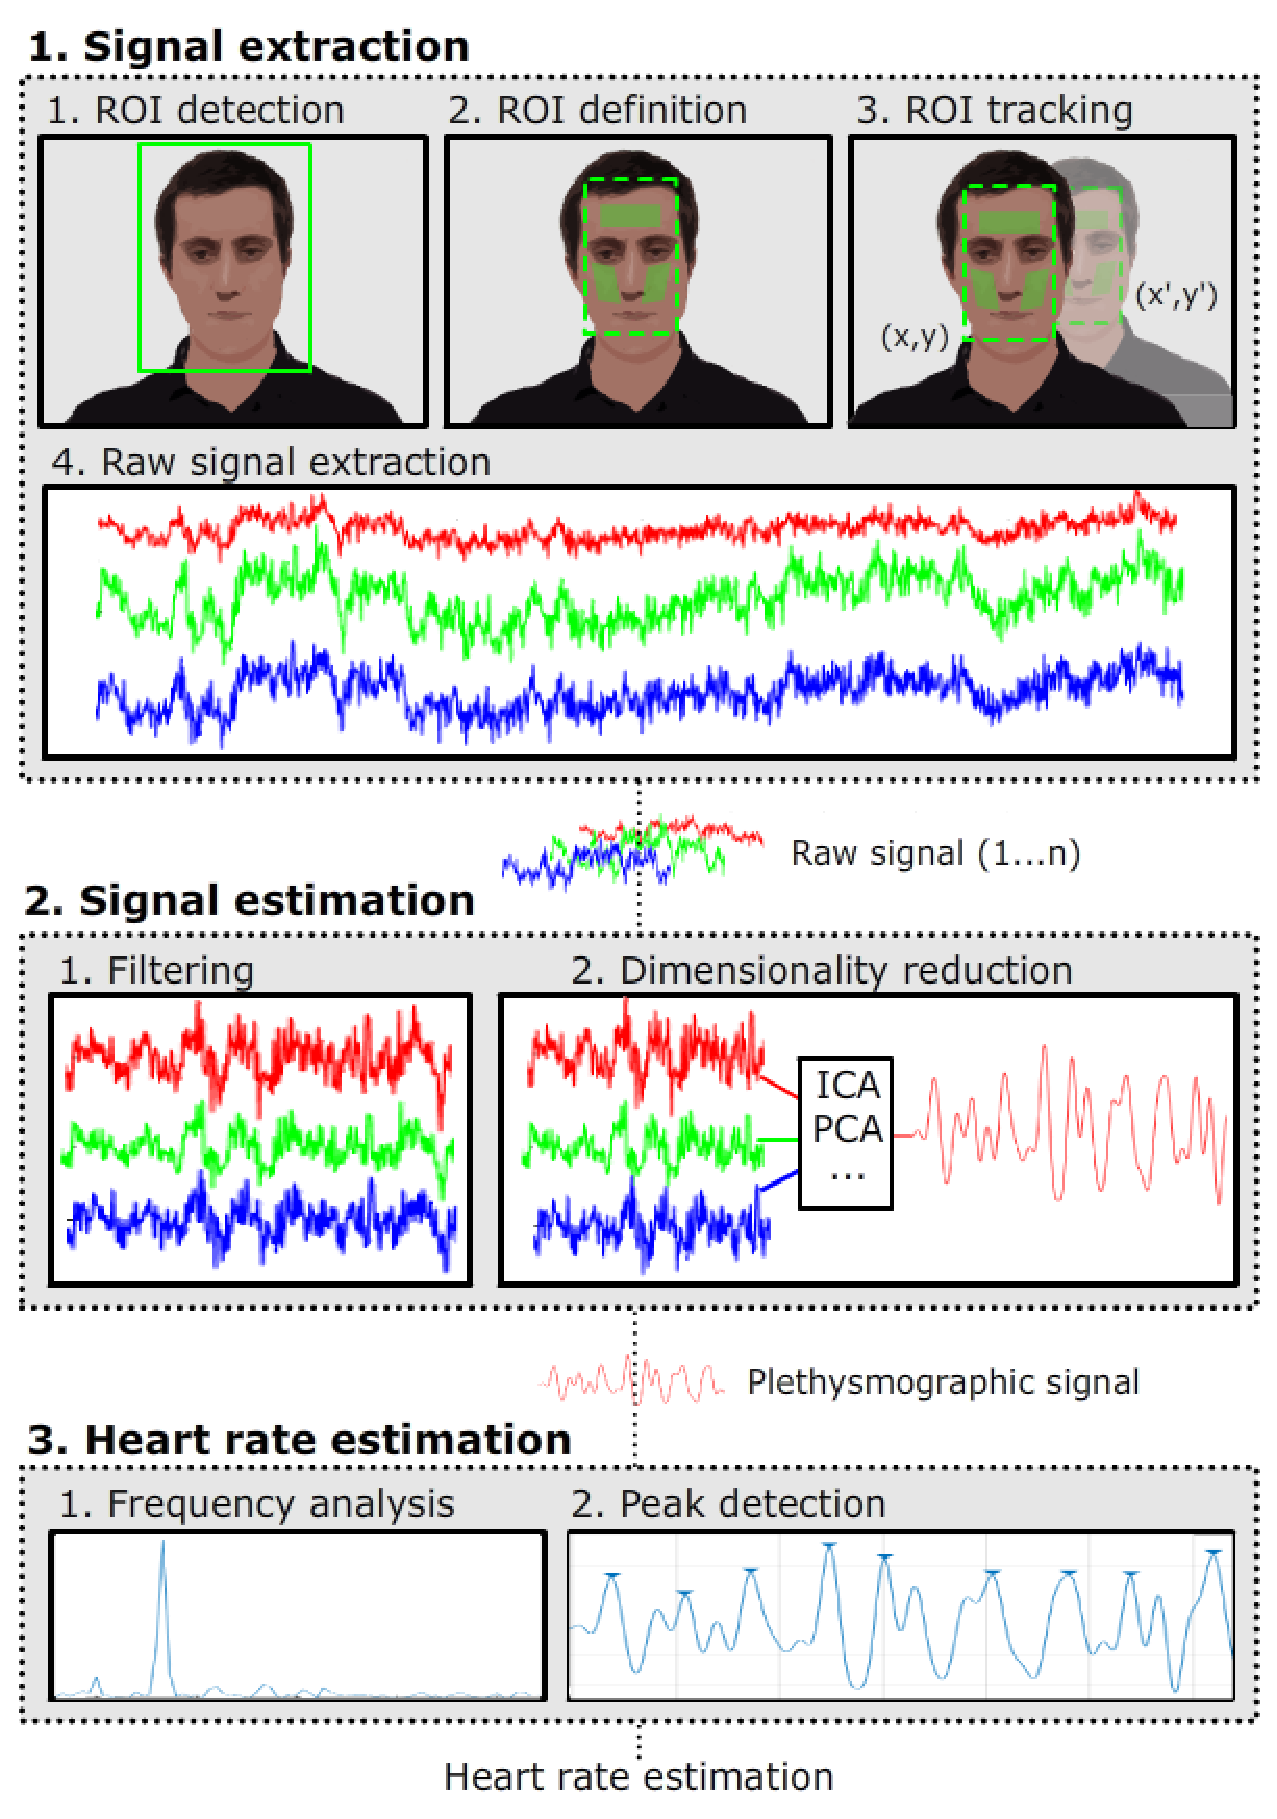
\includegraphics[width=0.9\linewidth]{Content/figures/general-rppg}
\caption{General algorithm framework common to all rPPG techniques. Adapted from \textcite{rouast2016remote}.}
\label{fig:rppg}
\end{figure}

\subsection{Signal extraction}

The signal extraction phase extracts a set of raw signals from a video. Step 1 relates to the detection of a region of interest (ROI), which is an area of the video that usually contains the face of the subject. Approaches commonly used for this step are the VJ\footnote{VJ is the abbreviation of \textit{Viola \& Jones}, which is how the algorithm is commonly mentioned in the literature.} algorithm of \textcite{viola2004robust}, a machine learning based approach to classifying faces, Active Appearance Models (AMM) \parencite{EdwardsAAM} and facial landmark detectors. %\parencite{saragih2011deformable,martinez2013local}.

In step 2 (ROI definition) the parts of the ROI to be used for the signal extraction are defined. Approaches commonly employed include the use of whole ROI (usually the bounding box returned by VJ, which is likely to contain background pixels along with the facial pixels), a part of the ROI (e.g. 60\% of the bounding box width) or specially defined areas (e.g. forehead, cheeks or shapes defined by facial landmark points).

Step 3 (ROI tracking) deals with the process of tracking the defined ROI area over the duration of the video. Ideally the PPG signal should be extracted from the pixels belonging to the same skin region over time. This is unlikely to happen due to subject motion, be it voluntary or not (subjects will present movement that influences the ROI even when still \parencite{poh2010non}). A common approach for this step is the re-detection of the ROI for each frame, which is computationally suboptimal and still prone to noise. Detection algorithms, e.g. VJ, are not likely to be exact, so results between consecutive frames might be slightly different, which causes fluctuation in the defined ROI. More elaborated approaches avoid the costly frame-by-frame re-detection procedure (and its fluctuations) by updating an already detected ROI in subsequent frames. The update is based on movement information obtained from tracking algorithms applied to features/points within the ROI. %Examples of such algorithms are Good Features to Track, Kanade-Lucas-Tomasi (KLT), Speeded Up Robust Features (SURF), Kernel-based Object Tracking and tracking-by-detection with kernels.

Finally in step 4 (raw signal extraction) a raw (untreated) signal is extracted. It is a time-varying signal whose points/samples are obtained from the content of the defined ROI in each frame of the video. One common approach used to extract the signal is based on colors, e.g. average of the values of the pixels of each channel (R, G and B) over time produces the raw signal. Another approach is based on the movement of the head, which is a mechanical reaction to the blood flow in the aorta. Feature points within the defined ROI are tracked over time by a tracking algorithm and the horizontal and/or vertical variations in the trajectory of the points produce the raw signal. The signal extraction phase can result in multiples raw signals, which are dependent on the approach applied. A color-based approach, for instance, might result in three raw signals, one for each color channel (RGB).

\subsection{Signal estimation}

The raw signals are filtered and combined to produce a single estimated plethysmographic signal. The filtering step aims to remove unwanted noise from the raw signal, which could be caused by the capturing device (e.g. camera noise), subject movement, changes in illumination, etc. The raw signal is usually normalized (subtracted by its mean and divided by its standard deviation) first. The commonly used filters are based on high/low pass, such as bandpass, moving average window and detrending based on Smoothness Priors Approach (SPA) \parencite{eleuteri2012efficient}. Since the feasible frequencies for the HR band are known, filters are usually configured to eliminate frequencies outside that band, e.g. cutoff frequencies of [0.7 Hz, 4.0 Hz], which eliminates from the raw signal frequencies outside the [42 bpm, 240 bpm] interval.

In the dimensionality reduction step, the raw signal is used to estimate the plethysmographic signal, i.e. the one containing the HR. As previously mentioned, depending on the approach used for the raw signal extraction, one or more raw signals might be available for use in the estimation. One approach for the estimation is to simply choose one of the raw PPG signals as the estimated plethysmographic signal, e.g. the raw signal extracted from the G channel. Such choice is acceptable since the plethysmographic signal is known to be stronger in the green channel of an RGB video \parencite{verkruysse2008remote}, however it is more likely to contain noise since a raw (untreated) component is being used. Another approach relies on Blind Source Separation (BSS) methods, which tries to mitigate noise by assuming the estimated plethysmographic signal is a linear combination of the raw signals. Independent Component Analysis (ICA) \parencite{hyvarinen2000independent} and Principal Component Analysis (PCA) \parencite{jolliffe2002principal} are common BSS algorithms used to find the weight that each raw signal has in the linear combination to produce the estimated plethysmographic signal. Finally another approach assumes fixed weights for the linear combination, which are derived from models of skin illumination, for instance.

\subsection{Heart rate estimation}

Finally the estimated plethysmographic signal is analyzed and the HR is extracted. There are two steps in this phase, frequency analysis and peak detection, however only a single one of them is usually performed. In the frequency analysis step, approaches include Continuous Wavelet Transform (CWT) used to construct a time-frequency representation of the plethysmographic signal, and Fourier Transform to analyze the signal in the frequency domain. Regarding the later, the estimated plethysmographic signal is assumed to contain a distinct periodicity (the HR). As a result, when converted into the frequency domain via Fast Fourier Transform (FFT), for instance, the signal should present a high spectral power associated with the frequency of such distinct periodicity. As a consequence, the index of the frequency with the highest peak in the power spectra in the frequency domain corresponds to the HR.

In the peak detection step, however, the signal is not converted into the frequency domain, instead it is interpolated and peaks are detected (usually with a local maxima algorithm). The distances among the peaks correspond to the inter-beat interval (IBI), which is then used to calculate the HR (as $60/\overline{IBI}$) and/or the heart rate variability (HRV).

%%%%%%%%%%%%%%%%%%%%%%%%%%%%%%%%%%%%%%%%%%%%%%%%%%%%%%%%%%%%%%%%%%%%%%%%%%%%%%%%%%%%%%%%%%%%%%%%%%%%%%%
\section{Consolidated techniques}
\label{sec:literature-rppg-techniques}
%%%%%%%%%%%%%%%%%%%%%%%%%%%%%%%%%%%%%%%%%%%%%%%%%%%%%%%%%%%%%%%%%%%%%%%%%%%%%%%%%%%%%%%%%%%%%%%%%%%%%%%

The previously described general algorithm framework for rPPG techniques illustrates the wide range of variations possible by different combinations of approaches within each step of the process. Early initiatives regarding rPPG, for instance, used manually detected/defined ROI, few or no use of signal filtering and signal extraction based on the average of image brightness \parencite{takano2007heart} or colors \parencite{verkruysse2008remote}.
%Additionally the authors presented findings regarding the process: PPG signal is stronger in the green channel of an RGB video, which is aligned with the fact that hemoglobin absorbs green light better; each pixel in the ROI contributes to the HR signal detection, which implies that the selection/size of the ROI is not critical for HR determination; lighter areas in the video often feature a higher pulse signal; and the PPG signal obtained from facial regions, specially the forehead, are stronger than other body parts.

The work of \textcite{poh2010non} was the first in the field to rely on BSS. Figure \ref{fig:poh} illustrates the proposed approach. The authors extracted the signal using automatic definition/tracking of the ROI (based on 60\% width of a VJ bounding box) and the average of the color channels. The three raw signals (derived from R, G and B) were filtered, detrended and decomposed using ICA. The second component generated by ICA was interpolated and a custom algorithm detected peaks to identify the HR. The authors further improved the technique by selecting the ICA component whose power spectrum contained the highest peak \parencite{poh2011advancements} and by incorporating alternate frequency bands (i.e. orange and cyan) into the extraction phase \parencite{mcduff2014improvements}.

\begin{figure}
\centering
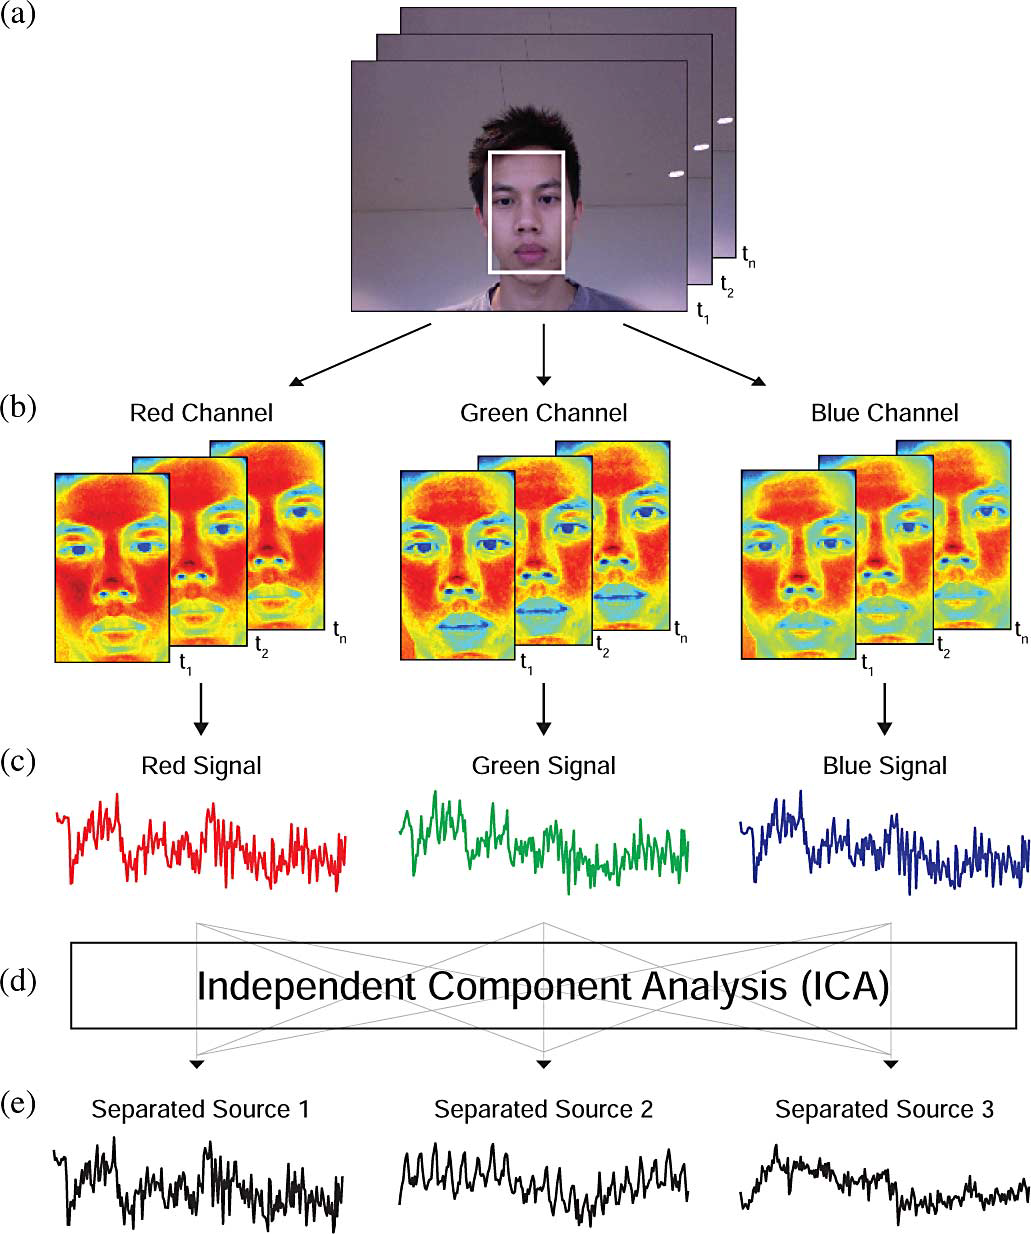
\includegraphics[width=0.6\linewidth]{Content/figures/poh.png}
\caption{Overall structure of rPPG approach based on ICA. Adapted from \textcite{poh2010non}.}
\label{fig:poh}
\end{figure}

\textcite{Datcu_2013} present a similar approach, however using AAM to segment the face of the subject into ROIs. \textcite{li2014remote} also use a different ROI, based on facial landmarks, and a combination of additional steps to mitigate noise caused by illumination, motion and facial expressions by removing signal outliers. \textcite{bousefsaf2013continuous} propose a variation of the previously described approaches, using a skin detection procedure to select pixels in the signal extraction phase. Additionally CWT is used in the signal estimation phase instead of the commonly used FFT, which is pointed by authors as more suitable for rapid changes in frequencies in time. As a consequence, the authors were able to detect the instantaneous HR (iHR) and significantly reduce the waiting time for the detection of HR measurements.

%used a digital version of the Stroop test and a video of a subject (captured by a webcam) to calculate HR and HRV to detect stress. A combination of HR, HRV and $HRV_{HF}$ is used to estimate the stress state. The resulting stress state curve tends to decrease during the rest period and increase during stress sessions (as the HR measurements), in accordance with previously mentioned works; additionally self-reported answers from questionnaires present significant differences of stress level in the rest and in the stress sessions as well, which confirms that remote reading and processing of HR as an input signal is able to relate with the real emotional state of an user. The detection mechanism, however, is purely based on the assumption that stress increases the HR mean. Both HR and HRV are averaged and interpolated within a time span (27 seconds) and the resulting wave produced from that calculation is said to be the stress level. Such wave might describe stress levels, since it matched variations of electrodermal response (EDR) data recorded using a skin conductance sensors, which is an indicator of stress, but the wave can also be seen as a simple representation of the HR and HRV variations, not stress itself.

Different approaches that are not based on the average of colors of the face can also be found in the literature. Those techniques use knowledge of the color vector of the different components to perform  the signal extraction. \textcite{Wang_2016novel} focus on the definition of a plane orthogonal to the skin-tone, ignoring pixels outside the subspace of skin pixels in the signal estimation phase. Similarly \textcite{de_Haan_2013} also use a skin model to generate a chrominance-based PPG signal, which is calculated as a combination of the intensities of the color channels in the video instead of their average. Those techniques aim to be more resilient than BSS-based techniques regarding motion noise. \textcite{6619284} are the first to completely move away from color-based initiatives and perform the signal extraction based on head movements. \textcite{Irani} further improved the technique by using a moving average filter applied to the trajectory of the feature points being tracked to remove the noise produced by other sources of motion, e.g. respiratory activity.
%Yun et al. \parencite{yun2009game}, on the other hand, demonstrated that changes in HR cause variation of temperature in the lower area of the forehead, which can be measured by a thermal imaging camera and used to infer stress state. The analysis performed by the authors was based on the variations of temperature in such lower area of the forehead, which differs from the color averaging approach previously described and used by other authors. The results, however, highlight that the region is affected by stress activities, which confirms the findings of \parencite{Datcu_2013}, \parencite{Sereevoravitgul} and \parencite{verkruysse2008remote} that point the forehead area as being more prone for remote readings.

The different settings in each phase of an rPPG technique result in a trade-off between advantages and disadvantages. Estimation based on head movement, e.g. \textcite{6619284}, does not rely on previous knowledge about colors nor requires visible skin area to work. However it is outperformed by other methods when subjects are not completely still \parencite{li2014remote} since it is significantly affected by subject motion. Techniques based on pre-defined skin-tone models, e.g. \textcite{Wang_2016novel,de_Haan_2013}, better adapt to changes in illumination (including non-white light sources), however they suffer performance degradation when the skin mask is not properly defined (or is noisy) or the pre-defined skin model is inaccurate \parencite{Wang_2016algorithmic}. Finally BSS-based methods, e.g. \textcite{poh2011advancements}, rely on BSS techniques (e.g. ICA) which are ideal to de-mix the estimated PPG signal from noise. However such techniques are unable to deal with periodic motion (i.e. exercise situation) and its statistical nature requires a long signal to enable an accurate measurement \parencite{Wang_2016algorithmic}. Despite such limitations, the ICA-based rPPG technique by \textcite{poh2011advancements} presents the best signal-noise ratio (SNR) for HR estimation under stationary situations (i.e. non-exercising) with different illumination conditions when compared to other techniques \parencite{Wang_2016novel}. The work is also extensively cited in the literature and often used as a benchmark for new techniques, which makes it a consolidated and robust solution.

%%%%%%%%%%%%%%%%%%%%%%%%%%%%%%%%%%%%%%%%%%%%%%%%%%%%%%%%%%%%%%%%%%%%%%%%%%%%%%%%%%%%%%%%%%%%%%%%%%%%%%%
\section{Accuracy and limitations}
%%%%%%%%%%%%%%%%%%%%%%%%%%%%%%%%%%%%%%%%%%%%%%%%%%%%%%%%%%%%%%%%%%%%%%%%%%%%%%%%%%%%%%%%%%%%%%%%%%%%%%%

The structure of rPPG techniques, as previously described, requires the analysis of each frame of a video to estimate the HR. As a consequence, any rPPG technique is influenced by the frame rate of the video, which accounts for the number of frames displayed per second (expressed in frames per second, or FPS), the resolution of each of those frames and the number of subsequent frames required to allow an estimation.

The frame rate of the video used in the estimation is directly connected to the sampling frequency, named $F_s$. Assuming that all frames of a video are used by an rPPG technique, a video running at 30 FPS allows a $F_s$ of 30 Hz, since each frames generates a sample. The minumum FPS required for the estimation must adhere to the Nyquist limit, which states that the sampling frequency must be at least twice as high as the highest frequency being measured:

\begin{equation*}
    F_s \geq 2 \cdot f_{Max}
\end{equation*}

where $f_{Max}$ denotes the highest frequency being measured. Since rPPG techniques are used to estimate HR, the value for $f_{Max}$ can be derived from a valid HR frequency interval. As previously described, a normal person presents a HR between the interval [45 bpm, 240 bpm], which is equivalent to the interval of [0.75 Hz, 4 Hz]. As a consequence, $f_{Max}$ is 4Hz (240 bpm) and $F_s$ is calculated as $F_s \geq 2 \cdot 4$, resulting in a minumum $F_s$ of 8 Hz, which translates to a video with frame rate of 8 FPS.

A fourier transform, e.g. FFT, is usually employed in rPPG techniques. The FFT divides the frequency spectrum of the input signal into $N$ number of discrete frequency blocks equal to the number of samples in the input signal. The number of samples $N$ used for the estimation is commonly refered to as window size. The smallest frequency that can be differentiated within that spectrum is named frequency resolusion, $\Delta f$, which is calculated as:

\begin{equation}
    \Delta f = \frac{F_s}{N}
    \label{eq:frequency-resolution}
\end{equation}

The frequency resolution $\Delta f$ influences the error rate in the estimation of the HR. For instance, if $\Delta f$ is 0.1 Hz, the HR will be estimated with an error of $\pm 3$ bpm. A low HR estimation error is desired, so a low value for $\Delta f$ is desired as well. By analysis of equation \ref{eq:frequency-resolution}, it is noted that $\Delta f$ descreases when $F_s$ descreases or when $N$ increases.

The value for $F_s$ is usually dependent on the camera device being used, which follows certain standards, e.g. 30 FPS. As a consequence, $\Delta f$ can be altered by changes on the window size $N$. Such changes, however, directly impact the estimations, since there is a trade-off between the window size and the estimation error. The higher the window size, the longer the video segment required for the estimation. Longer video segments are likely to contain movement of the subject being analyzed, which adds noise to the rPPG estimation.

\begin{table}[h!]
\caption{Frequency resolution $\Delta f$ (in Hz) as a function of window size (in samples) and frame rate (in FPS) \parencite{roald2013estimation}.}
\label{table:frequency-resolution}
\centering
\begin{tabular}{ccccccc}%
\toprule%
\textbf{Window size} & \textbf{10 FPS} & \textbf{15 FPS} & \textbf{25 FPS} & \textbf{30 FPS} & \textbf{50 FPS} & \textbf{60 FPS} \\
\midrule
100 & 0.1 & 0.15 & 0.25 & 0.3 & 0.5 & 0.6 \\
200 & 0.05 & 0.075 & 0.125 & 0.15 & 0.25 & 0.3 \\
300 & 0.033 & 0.05 & 0.083 & 0.1 & 0.17 & 0.2 \\
400 & 0.025 & 0.037 & 0.062 & 0.075 & 0.12 & 0.15 \\
500 & 0.02 & 0.03 & 0.05 & 0.06 & 0.1 & 0.12 \\
600 & 0.017 & 0.025 & 0.042 & 0.05 & 0.08 & 0.1 \\
700 & 0.014 & 0.02 & 0.03 & 0.04 & 0.07 & 0.08 \\
1000 & 0.01 & 0.015 & 0.025 & 0.03 & 0.05 & 0.06 \\
\bottomrule%
\end{tabular}%
\end{table}

\textcite{roald2013estimation} presents this trade-off by detailing the frequency resolution as a function of window size and video frame rate, as demonstrated in Table \ref{table:frequency-resolution}. As an example, assuming a video of 50 FPS and a frequency resolution of 0.07 Hz (which corresponds to an estimation error of $\pm 2.1$ bpm), a window size of 700 samples is required (equivalent of a video segment of 14 seconds). Additionally it has been proven that limitations in the sampling frequency, e.g. low $F_s$, can be compensated in the PPG signal detection by the use of interpolation \parencite{sun2012noncontact}.
